% !TEX root = ./cvl.tex
\section{Experimental Results}
\label{sec:experimental}

\marcos{What are the goals of the experiments? Certainly related to performance breakdown, quality, scalability, showing feasibility of very large datasets.}
\marcos{Introduce hardware and software setup.}
\marcos{Say we use PostgreSQL + PostGIS here.}
\marcos{Say that automatic parallelism is not supported natively by PostGIS, but is an interesting avenue for future work.}
\marcos{Introduce datasets and any selection procedures to scale datasets with justification.}
\marcos{Show three/four main sections and plots, explain all of them, justify effects observed.}
\martin{Compare experimental results with theory e.g. expected approximation guarantee, number of constraints, number of records per constraint etc.}

Show performance, scalability and quality for algorithms and constraints, i.e. performance of "find conflicts" and "find set multicover".

\begin{figure}[htbp]
\begin{center}
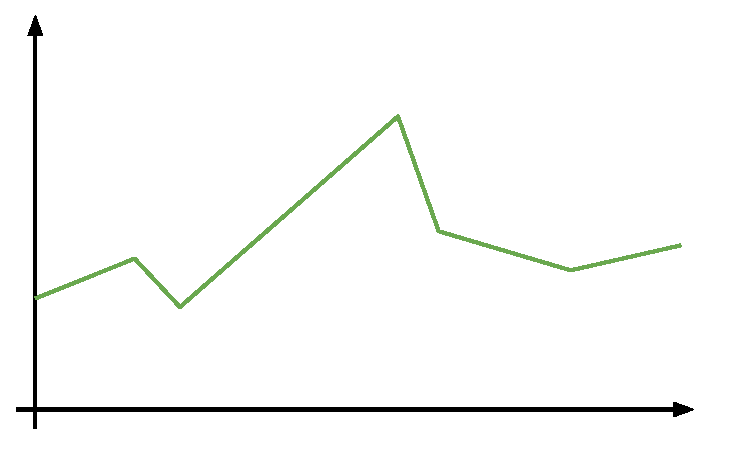
\includegraphics[scale=.5]{figs/cvl_todo.pdf}
\caption{Results for experiment.}
\label{fig:results-x}
\end{center}
\end{figure}

\begin{table}[htdp]
\caption{Datasets used in experiments}
\begin{center}
\begin{tabular}{|c|c|c|c|}
\hline
\textbf{Dataset} & \textbf{Type} & \textbf{Records} & \textbf{Points} \\
\hline
Openflights airports & Points & $7K$ & $7K$ \\
Tourist attractions & Points & $500K$ & $500K$ \\
Synthetic & Points & $30M$ & $30M$ \\
Danish Area Information & Polygons & $30K$ & $9M$ \\
US Waterways & Linestrings & $500K$ & $500K$ \\
\hline
\end{tabular}
\end{center}
\label{default}
\end{table}%
